% ★★ 中档
\newcommand{\qConicDefZeroPyramidStem}{
在三棱锥 $P-ABC$ 中，$PA=PB=PC=\sqrt{2}$，$AB=AC=BC=\sqrt{3}$，点 $Q$ 为 $\triangle ABC$ 所在平面内的动点，若 $PQ$ 与 $PA$ 所成角为定值 $\theta$，$\theta \in \left(0, \frac{\pi}{4}\right)$，则动点 $Q$ 的轨迹是（\quad）
}
\newcommand{\qConicDefZeroPyramidOptions}{
\mcoptions[4]{圆}{椭圆}{双曲线}{抛物线}
}
\newcommand{\qConicDefZeroPyramidFigure}{
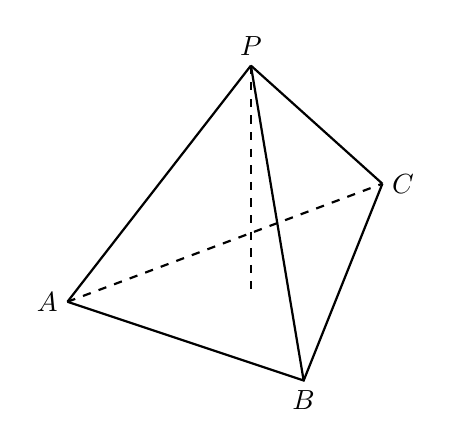
\begin{tikzpicture}[scale=1]
  \coordinate (A) at (0,0);
  \coordinate (B) at (3,-1);
  \coordinate (C) at (4,1.5);
  \coordinate (H) at (2.33,0.16); % approx centroid
  \coordinate (P) at (2.33, 3);
  \draw[thick] (A) -- (B) -- (C);
  \draw[thick, dashed] (A) -- (C);
  \draw[thick] (P) -- (A);
  \draw[thick] (P) -- (B);
  \draw[thick] (P) -- (C);
  \draw[thick, dashed] (P) -- (H);
  \node[left] at (A) {$A$};
  \node[below] at (B) {$B$};
  \node[right] at (C) {$C$};
  \node[above] at (P) {$P$};
\end{tikzpicture}
}
\newcommand{\qConicDefZeroPyramidAnswer}{
B
}
\newcommand{\qConicDefZeroPyramidSolution}{
作 $P$ 在平面 $ABC$ 内的投影 $H$。由于 $PA=PB=PC=\sqrt{2}$，可知 $H$ 为正三角形 $ABC$ 的外心。\\
对于正三角形 $ABC$，$AB=\sqrt{3}$，则其外接圆半径 $R = \frac{\sqrt{3}}{3} \times \sqrt{3} = 1$，即 $AH=1$。\\
在 Rt$\triangle PAH$ 中，$PA=\sqrt{2}$，$AH=1$，所以 $PH = \sqrt{(\sqrt{2})^2 - 1^2} = 1$。\\
于是 $\cos\angle PAH = \frac{AH}{PA} = \frac{\sqrt{2}}{2}$，所以 $PA$ 与平面 $ABC$ 所成角 $\beta = \frac{\pi}{4}$。\\
现 $PQ$ 与 $PA$ 所成角为 $\theta$，即动点 $Q$ 在以 $PA$ 为轴、半顶角为 $\theta$ 的圆锥面上。\\
因平面 $ABC$ 与轴 $PA$ 夹角为 $\beta = \frac{\pi}{4}$，且 $\theta \in \left(0, \frac{\pi}{4}\right)$，即 $\theta < \beta < \frac{\pi}{2}$，故截得的轨迹为椭圆。
}
